\documentclass[12pt,oneside,a4paper,english]{article}
\usepackage[T1]{fontenc}
\usepackage[margin=2.25cm,headheight=26pt,includeheadfoot]{geometry}
\usepackage[english]{babel}
\usepackage{listings}
\usepackage{color}
\usepackage{titlesec}
\usepackage{titling}
\usepackage[framed, numbered]{matlab-prettifier}
\usepackage{changepage}
\usepackage{amsmath}
\usepackage{hyperref}
\usepackage{enumitem}
\usepackage{graphicx}
\usepackage{fancyhdr}
\usepackage{lastpage}
\usepackage{caption}
\usepackage{tocloft}
\usepackage{setspace}
\usepackage{multirow}
\usepackage{titling}
\usepackage{float}
\usepackage{comment}
\usepackage{booktabs}
\usepackage{indentfirst}
\usepackage{lscape}
\usepackage{booktabs,caption}
\usepackage[flushleft]{threeparttable}
\usepackage[english]{nomencl}
\usepackage{xcolor}
\usepackage{lipsum}
\usepackage[utf8]{inputenc}
\usepackage{array}
\usepackage{multirow}
\usepackage{ragged2e}
\usepackage{multicol}


% --- set footer and header ---
\pagestyle{fancy}
\fancyhf{}

\setlength{\parindent}{2em}
\title{CDIO - Del 3} % to reference as \title, dont use \maketitle
\makeatletter\let\Title\@title\makeatother



\lstset{language=Matlab,
style=Matlab-editor,
basicstyle=\normalsize\mlttfamily,
numbers=left,
numberstyle={\scriptsize\color{black}},			% size of the numbers
numbersep=0.5cm											
}

\newlist{steps}{enumerate}{1}
\setlist[steps, 1]{leftmargin=1.5cm,label = Step \arabic*:}
\renewcommand{\headrulewidth}{1pt}
\renewcommand{\footrulewidth}{1pt}

%\lhead{\Title}
\rhead{\nouppercase{\rightmark}}
\lhead{\Title}
\rfoot{
\includegraphics[height=1.25cm]{root/logo.pdf}} % right header logo
\setlength\headheight{16pt}
\setlength{\footskip}{50pt}
\lhead{\Title} %rightH title
\cfoot{\thepage}

% --- End of page settings ---

\begin{document}
\pagenumbering{roman} 

\begin{titlepage}
\begin{center}
\vspace{2cm}
%\textsc{ Danmarks Tekniske Universitet}\\[1.5cm]

\includegraphics[width=0.4\textwidth]{root/dtu.png}~\\[1cm]
\vspace{2cm}

\vspace{2cm}

% Title
\hrule
\vspace{.5cm}
{ \huge \bfseries Title\\ of the report} % title of the report
\vspace{.5cm}

\hrule
\vspace{1.5cm}

\textsc{\textbf{Authors}}\\
\vspace{.5cm}
\centering

% add your name here
student - sxxxxxx\\
student - sxxxxxx\\

\vspace{4cm}

\centering \today % Dags dato
\end{center}
\end{titlepage}

\newpage
\begin{flushleft} % sætter tekststarten i venstre marginside.

\doublespacing

In the present project, we developed a Monopoly Junior game for Windows OS users. The project followed a Unified Process style of workflow including the following two phases: elaboration and construction. The analyses for the project included a requirements specification, actor and use-case analyses and a domain analysis. The designs for the project included a system-sequence, sequence and design class analyses. The implementation resulted in a playable Monopoly Junior game with zero or undetected bugs. For tests, JUnit tests were conducted for each relevant software class along with a user test for the entier program. 

\end{flushleft}
\thispagestyle{fancy}

\newpage
\doublespacing
%\addcontentsline{toc}{section}{Table of Contents}
\renewcommand{\baselinestretch}{1}\normalsize
\tableofcontents
\renewcommand{\baselinestretch}{1}\normalsize
%\singlespacing
\thispagestyle{fancy} % force page style



\newpage
\section{Timeregnskab}
\centering
\begin{tabular}{ |c|c|c|c|c|c|c|  }
 \hline
 \multicolumn{7}{|c|}{Timeregnskab (timer)} \\
 \hline
 Aktivitet & Lucas & Victor & Simon & Louis & Daniel & Isak\\
 \hline
 
 
 Programmering      & 0 & x & x & x & 16 & 15 \\
 
 Møder              & 6 & 4 & 4 & 4 & 8 & 8 \\
 
 Rapportskrivning   & 14 & 0.5 & 1 & x & x & x \\
 
 \hline
 
 I alt              & 20 & 4.5 & 5 & x & x & x \\
 
 
 \hline
\end{tabular}
\thispagestyle{fancy}
\pagenumbering{arabic} 
\fancyfoot[C]{Page \thepage\ of \pageref{endOfDoc}}



\newpage
\section{Introduktion}
\input{Report/sources/1_Introduction}
\thispagestyle{fancy}

\newpage
\section{Kravspecifikation}








\begin{center}
\begin{tabular}{ | c | c | } 
\hline
1 & Der skal kunne vælges mellem 2-4 spillere \\ 
\hline
2 & En spiller modtager 2 fra banken ved at lande på START \\ 
\hline
3 & Spillet skal kunne indlæse hver spillers alder \\ 
\hline
4 & Hver spiller starter på feltet start \\ 
\hline
5 & Hver spiller starter med 20, 18 eller 16 for hhv. 2, 3 eller 4 antal spillere \\ 
\hline
6 & Hvis der landes på et ikke-ejet felt betaler spilleren beløvet der står på feltet \\ 
\hline
7 & Hvis der landes på et ejet felt skal der betales det \\ 
\hline
8 & GUI'en skal implementeres i projectet \\ 
\hline
9 & x \\ 
\hline
10 & x \\ 
\hline
11 & x \\ 
\hline
12 & x \\ 
\hline
\end{tabular}
\end{center}
\thispagestyle{fancy}

\newpage
\section{Analyse}
\begin{flushleft}
\subsection{Fully dressed use-case}

\subsection{Casual use-cases}



\subsection{Domæne model}


\includegraphics[width=1\textwidth]{Report/figures/Domæne model CDIO del3.png}~\\[1cm]

\end{flushleft}
\thispagestyle{fancy}

\newpage
\section{Design}
\begin{flushleft}
\doublespacing
\subsection{Sekvensdiagram}
Med fodfæste i analysediagrammerne har vi udarbejdet et sekvensdiagram, der illustrerer de overordnede funktioner, der bliver udført af systemer, når man ruller med en terning, rollDice(se figur 5.1.1). Her kaldes altså på metoden diceRoll hos Dice, hvorefter der bliver returneret terningernes øjne. Herefter kalder Game på getPosition hos Player, der returnerer den nuværende spillers position, hvorefter der udregnes en ny position. Når den nye position er fundet, kalder Game landOnField metoden hos Field, som er en abstrakt klasse - metoden er derfor polymorfisk. I følgende paragraffer beskrives hver polymorfisk case.Efter eksekvering af den landOnField tjekker Game for spillets regler hos Rules. Hvis en spiller har mindre en 0 stående på kontoen returnerer Rules en vinder. Herefter opdateres GUIen, hvor der til sidst skifter til næste spiller.
\addlinespace
For nedarvningen ChanceField (se figur 5.1.2) kalder ChanceField på drawChanceCard og executeChanceCard hos ChanceCard. Her trækkes altså et 'tilfældigt' kort, som eksekverer en handling. For at holde diagrammet simpelt viser vi ikke hvert chancekorts udførelse.
\addlinespace
For nedarvningen CustomField står en Player blot stille og der eksekveres altså ikke metoder (se figur 5.1.3).
\addlinespace
For nedarvningen JailField (se figur 5.1.4) kalder JailField på Player, som sætter Player i fængsel, isInJail = true. Hvis en Player ikke besidder et hasGetOutOfJailCard bliver der altså trukket penge fra Player's konto.
\addlinespace
For nedarvningen PropertyField (se figur 5.1.5) kaldes der på Account, setBalance, hvis feltet ikke allerede er købt - her købes feltet så og der trækkes prisen fra kontobalancen, Account. Hvis feltet er købt skal der betales leje, så der kaldes på setBalance hos Account med parametrene currentPlayer og owner, hvor der hhv. subtraheres og adderes med rent.
\addlinespace
I sidste nedarvning, StartField (se figur 5.1.6), kaldes på metoden addBalance hos Account, som tilfører currentPlayer 2 point til kontoen.
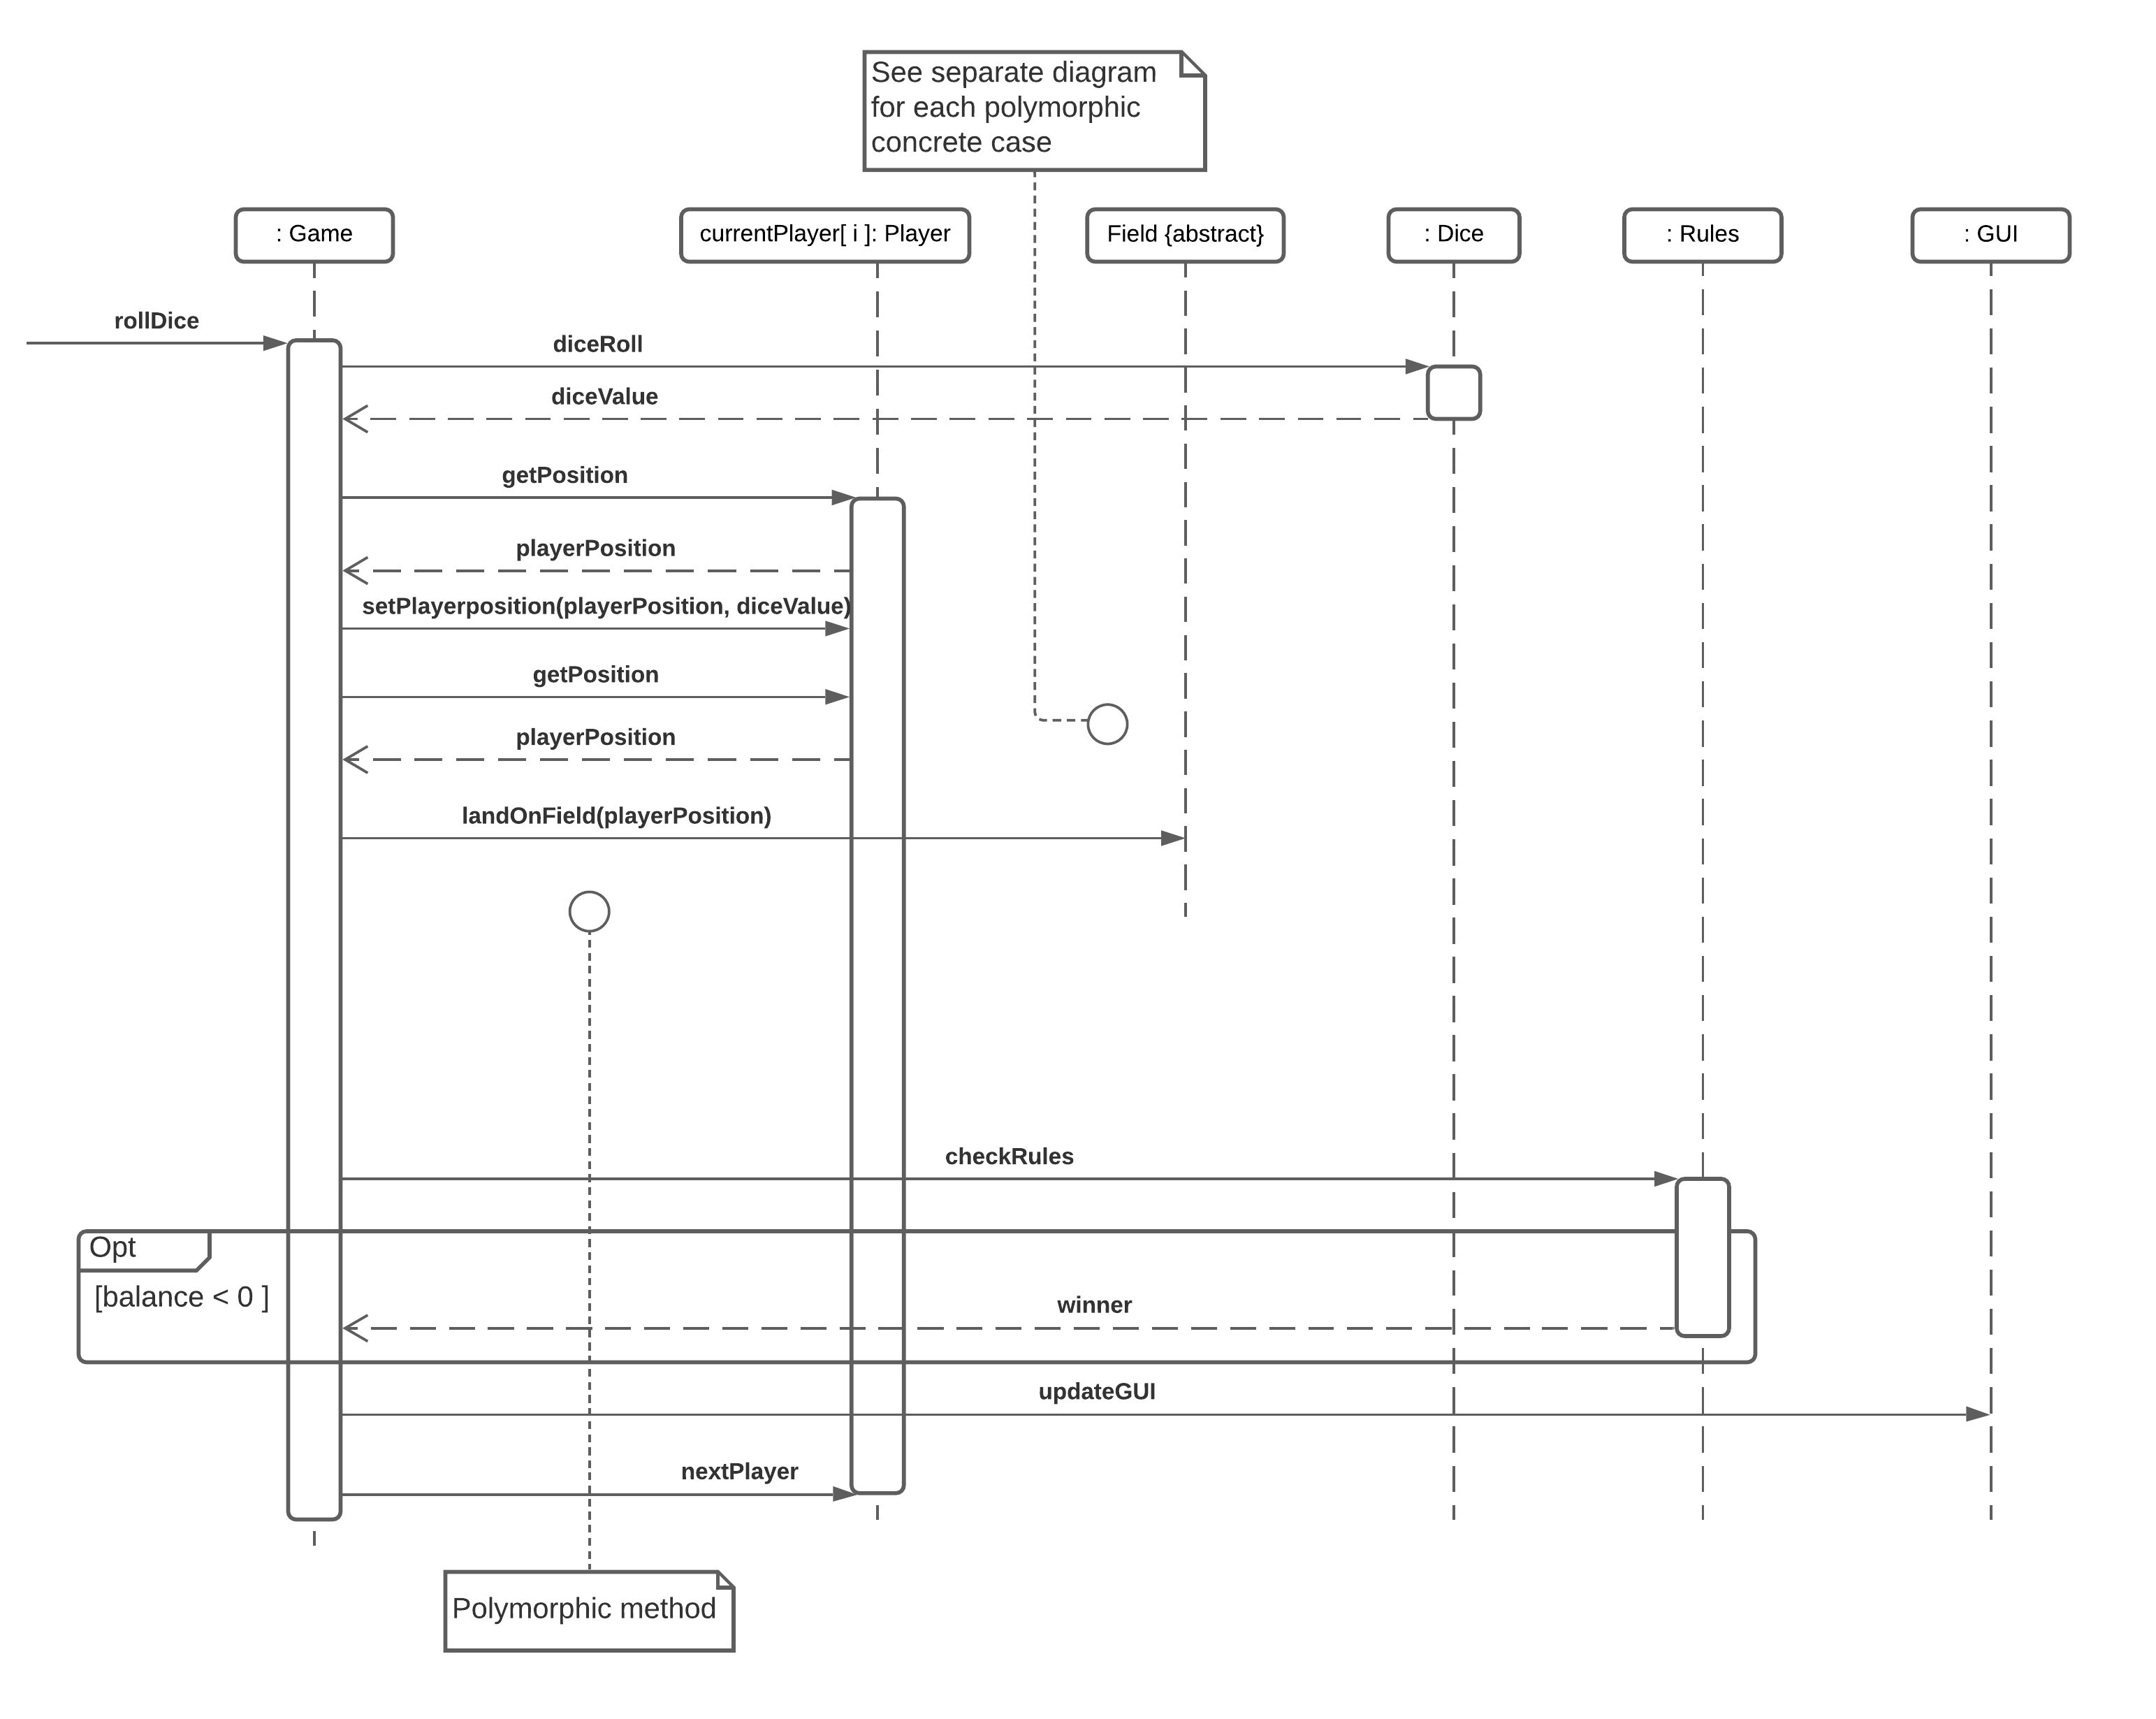
\includegraphics[width=1\textwidth]{Report/figures/Sekvensdiagram1.png}~\\[0cm]
Figur 5.1.1. Sekvensdiagram over rollDice som use-case.

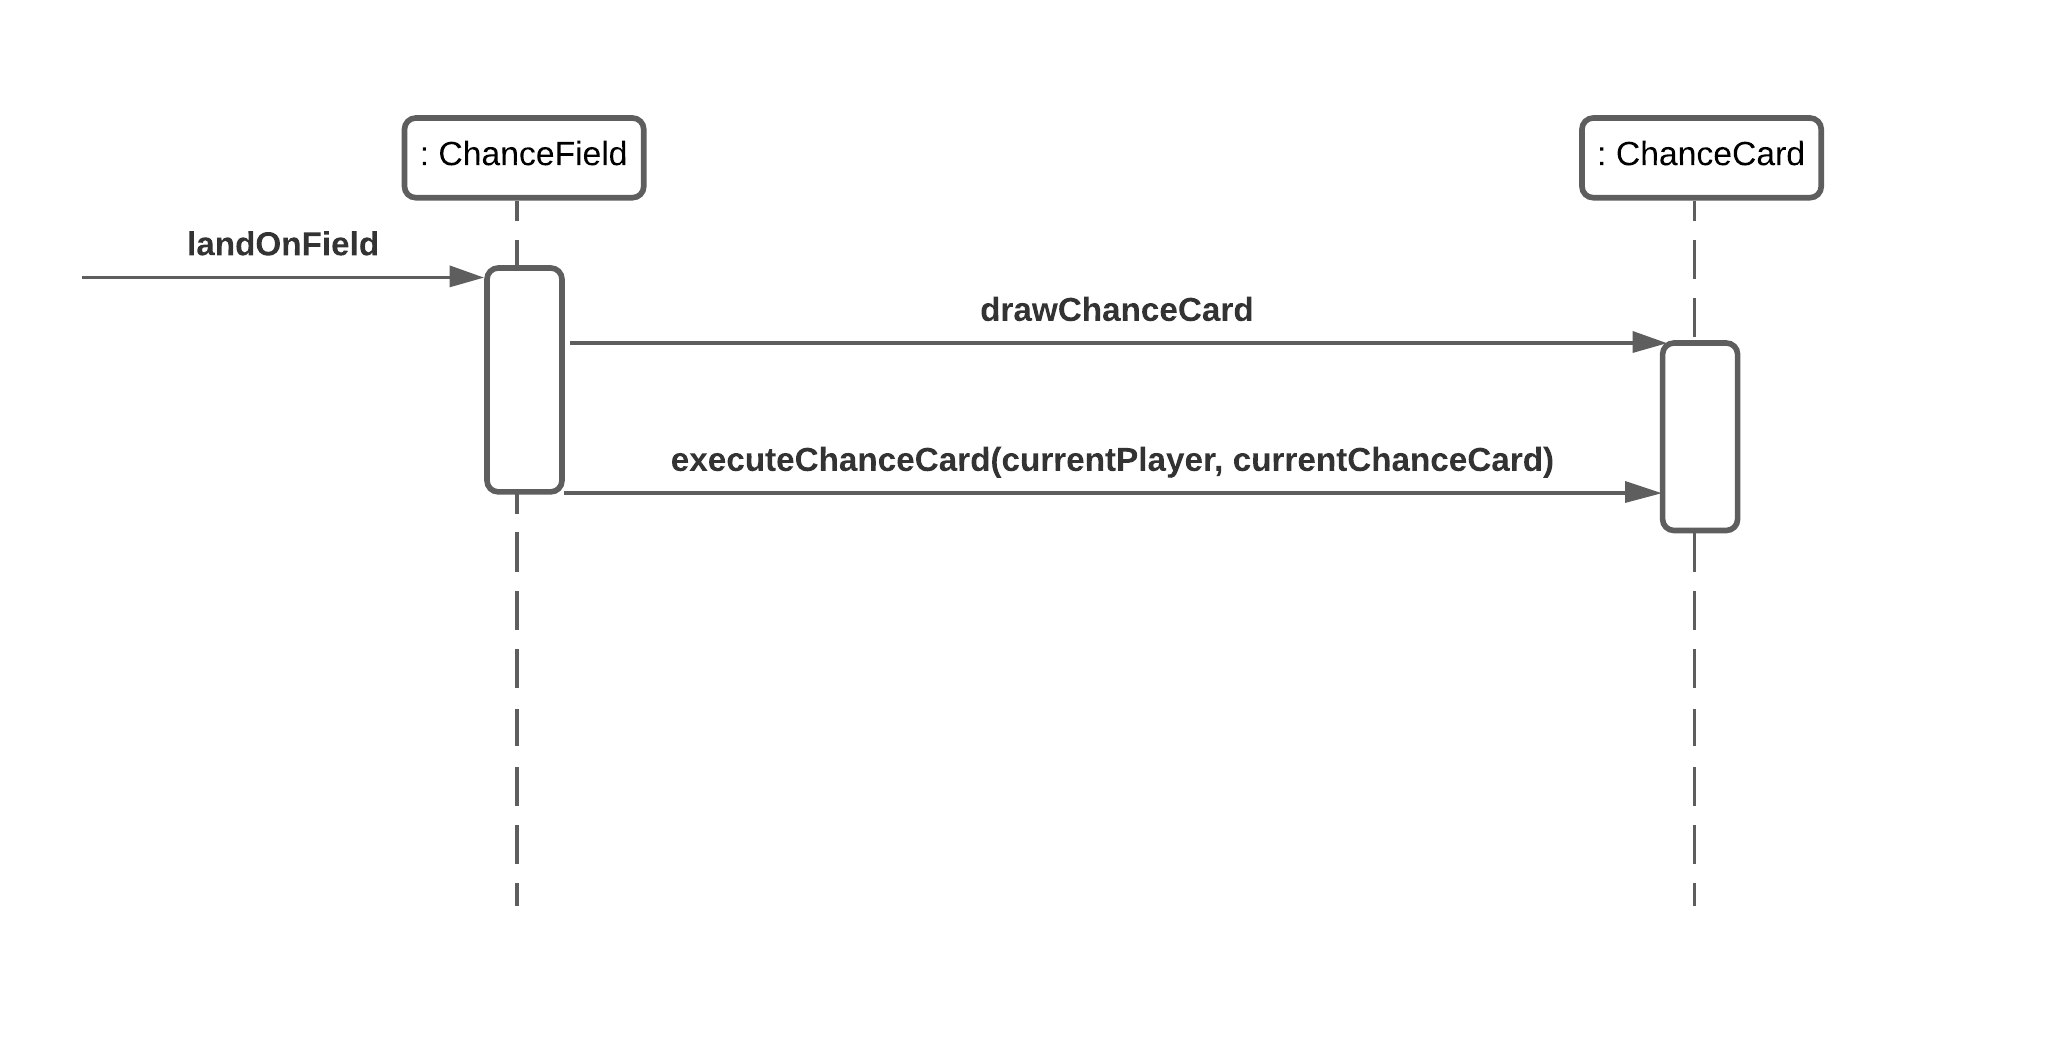
\includegraphics[width=0.9\textwidth]{Report/figures/Sekvensdiagram_ChanceField.png}~\\[0cm]
Figur 5.1.2. Sekvensdiagram over polymorphism af metoden landOnField for ChanceField.


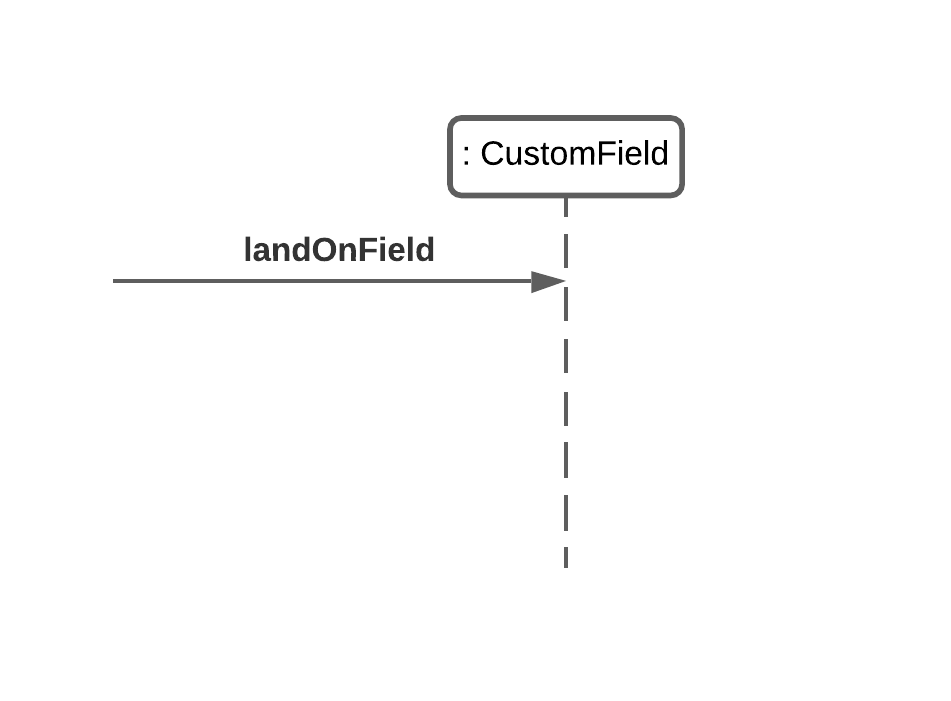
\includegraphics[width=0.9\textwidth]{Report/figures/Sekvensdiagram_CustomField.png}~\\[0cm]
Figur 5.1.3. Sekvensdiagram over polymorphism af metoden landOnField for CustomField.


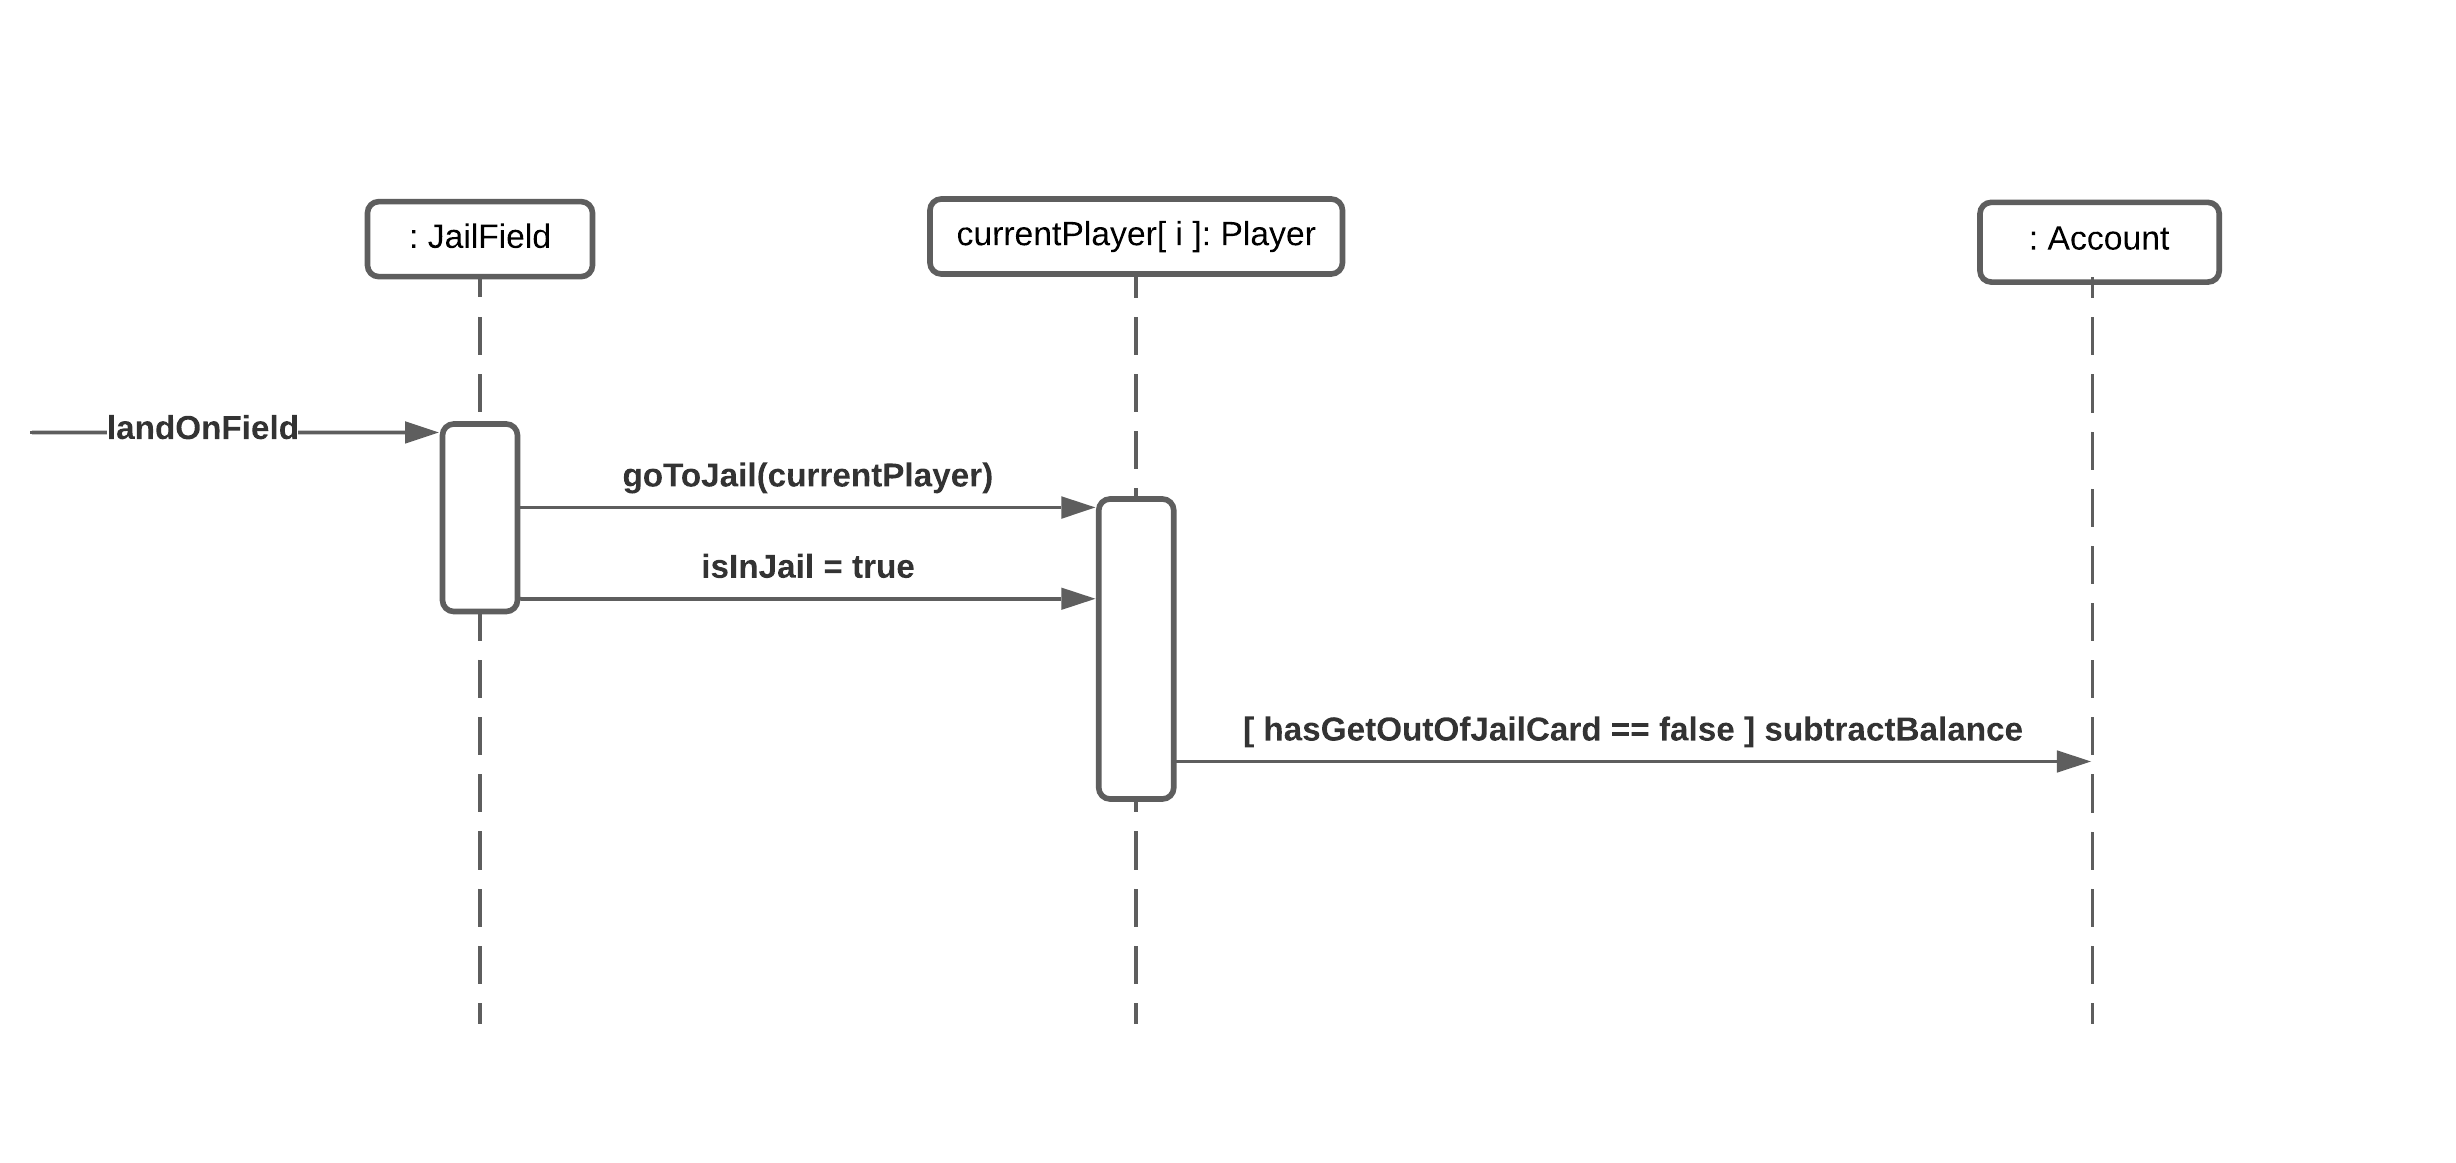
\includegraphics[width=0.9\textwidth]{Report/figures/Sekvensdiagram_JailField.png}~\\[0cm]
Figur 5.1.4. Sekvensdiagram over polymorphism af metoden landOnField for JailField.


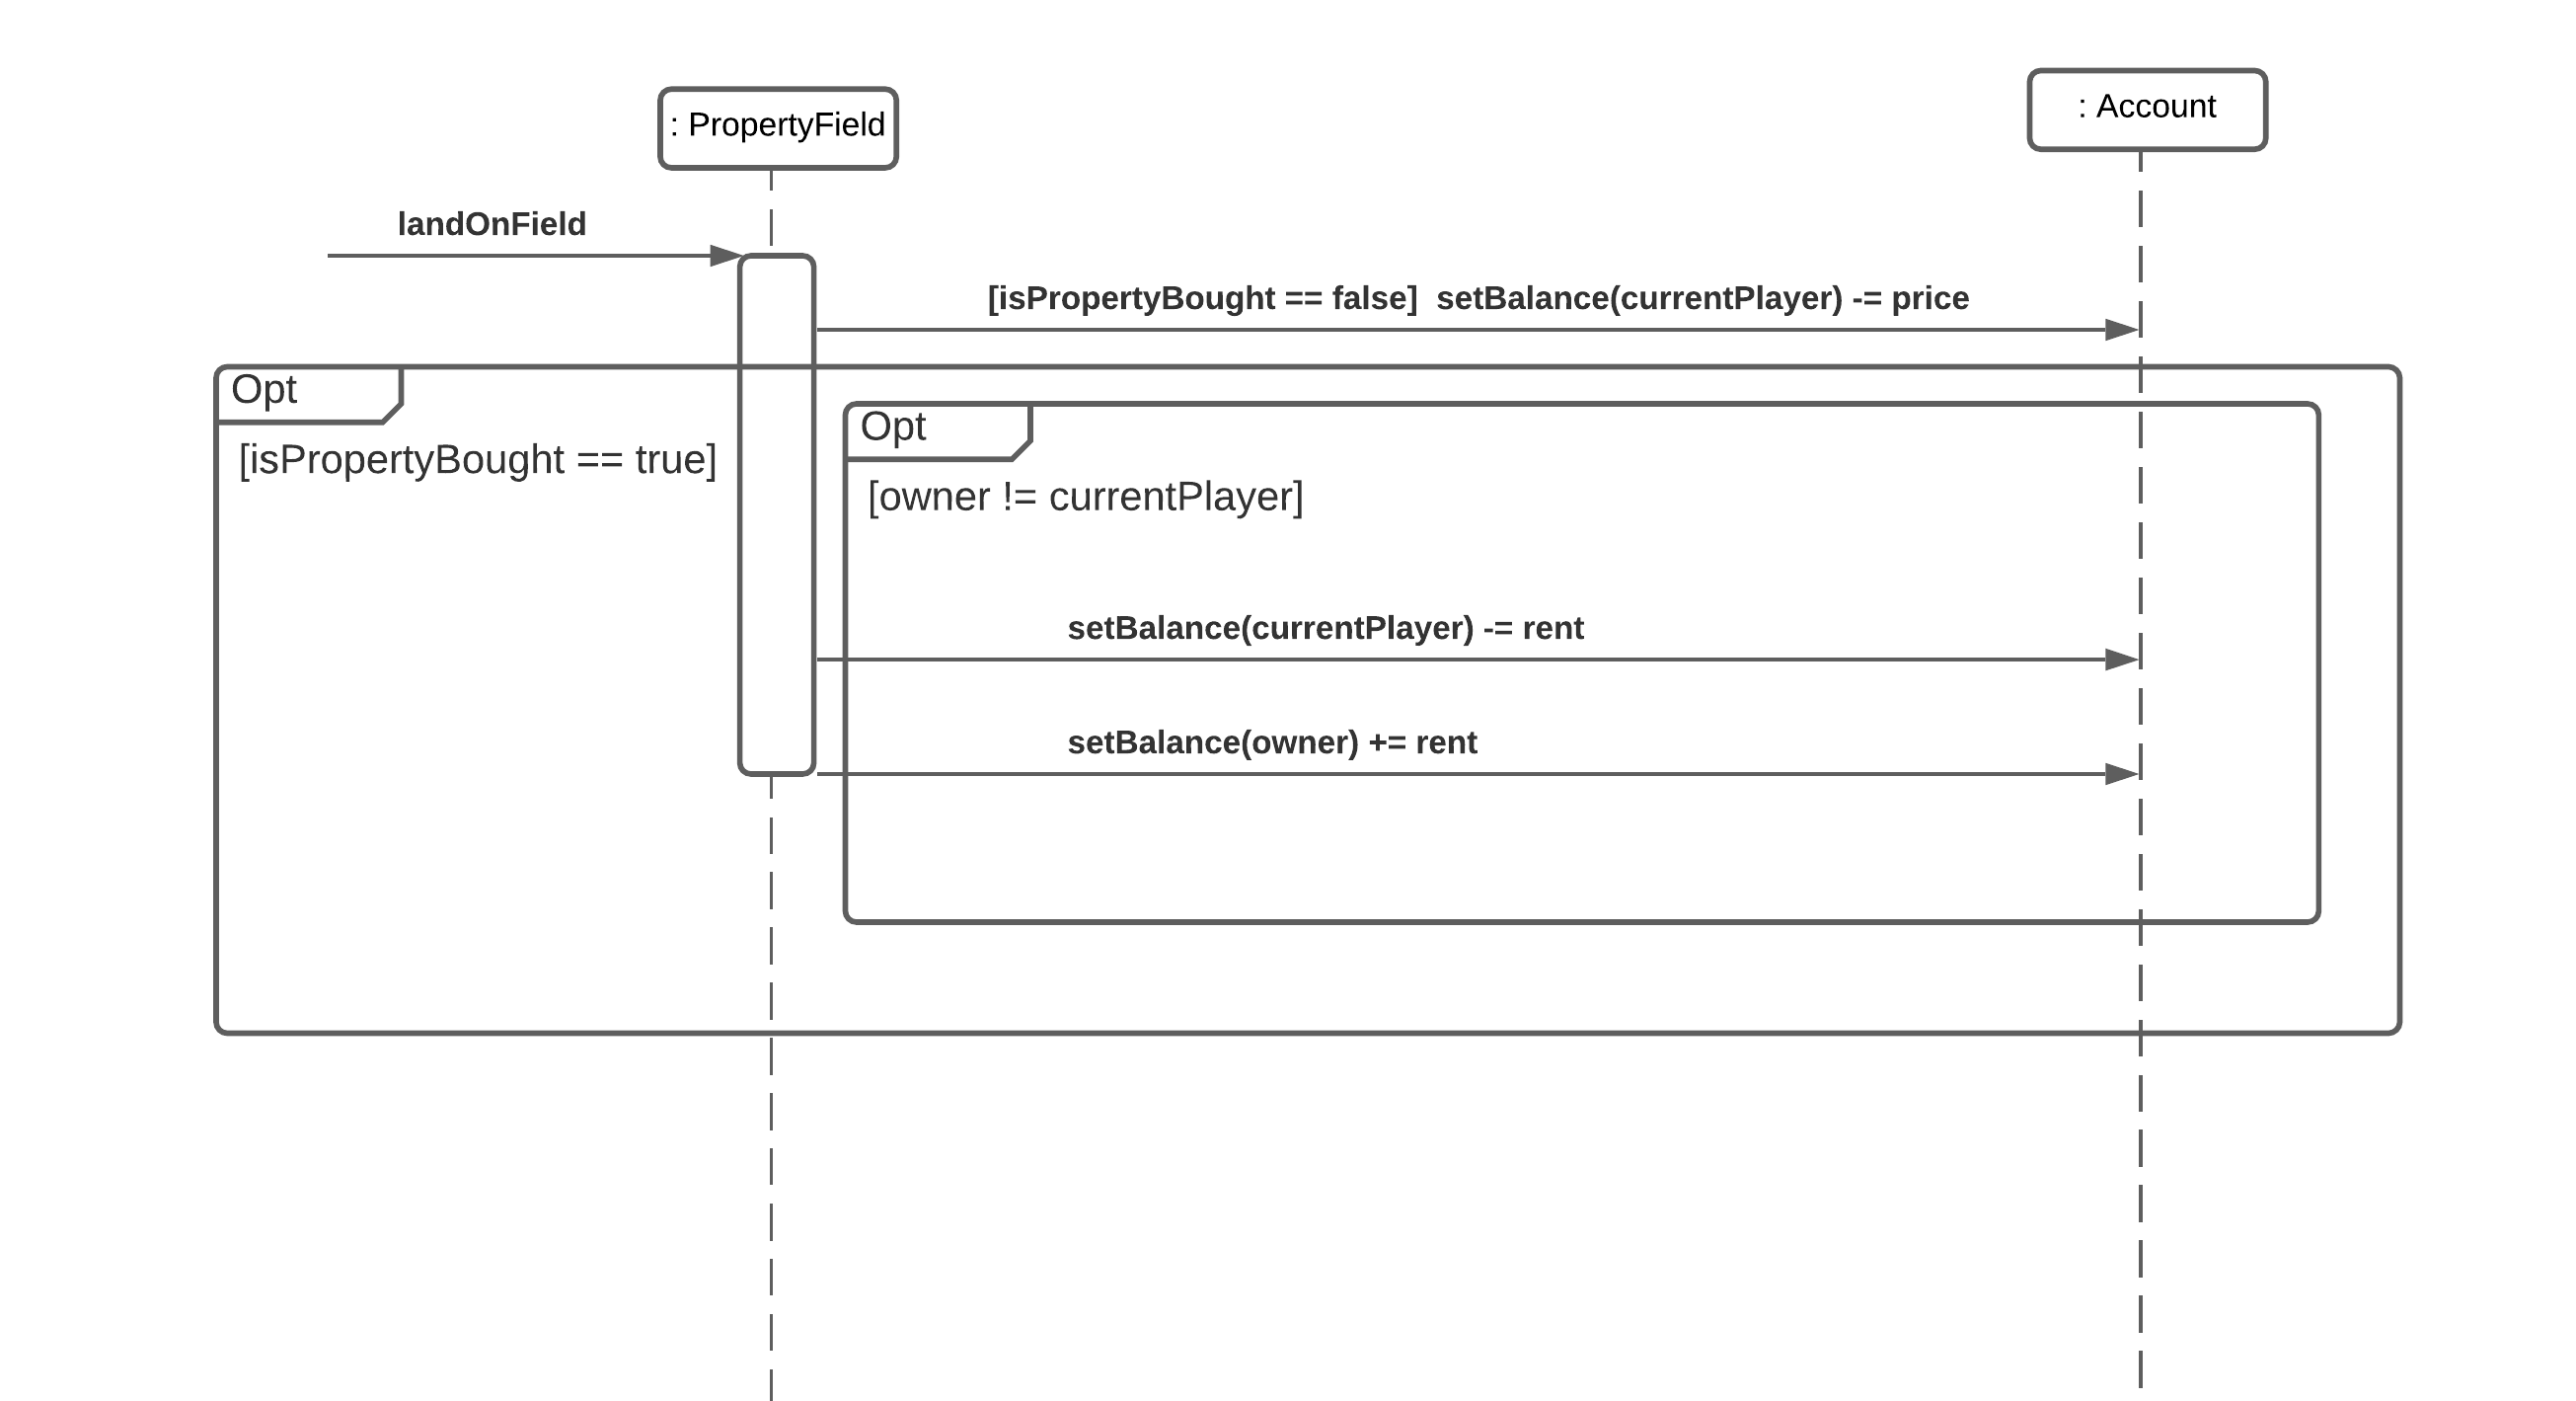
\includegraphics[width=0.9\textwidth]{Report/figures/Sekvensdiagram_PropertyField.png}~\\[0cm]
Figur 5.1.5. Sekvensdiagram over polymorphism af metoden landOnField for PropertyField.


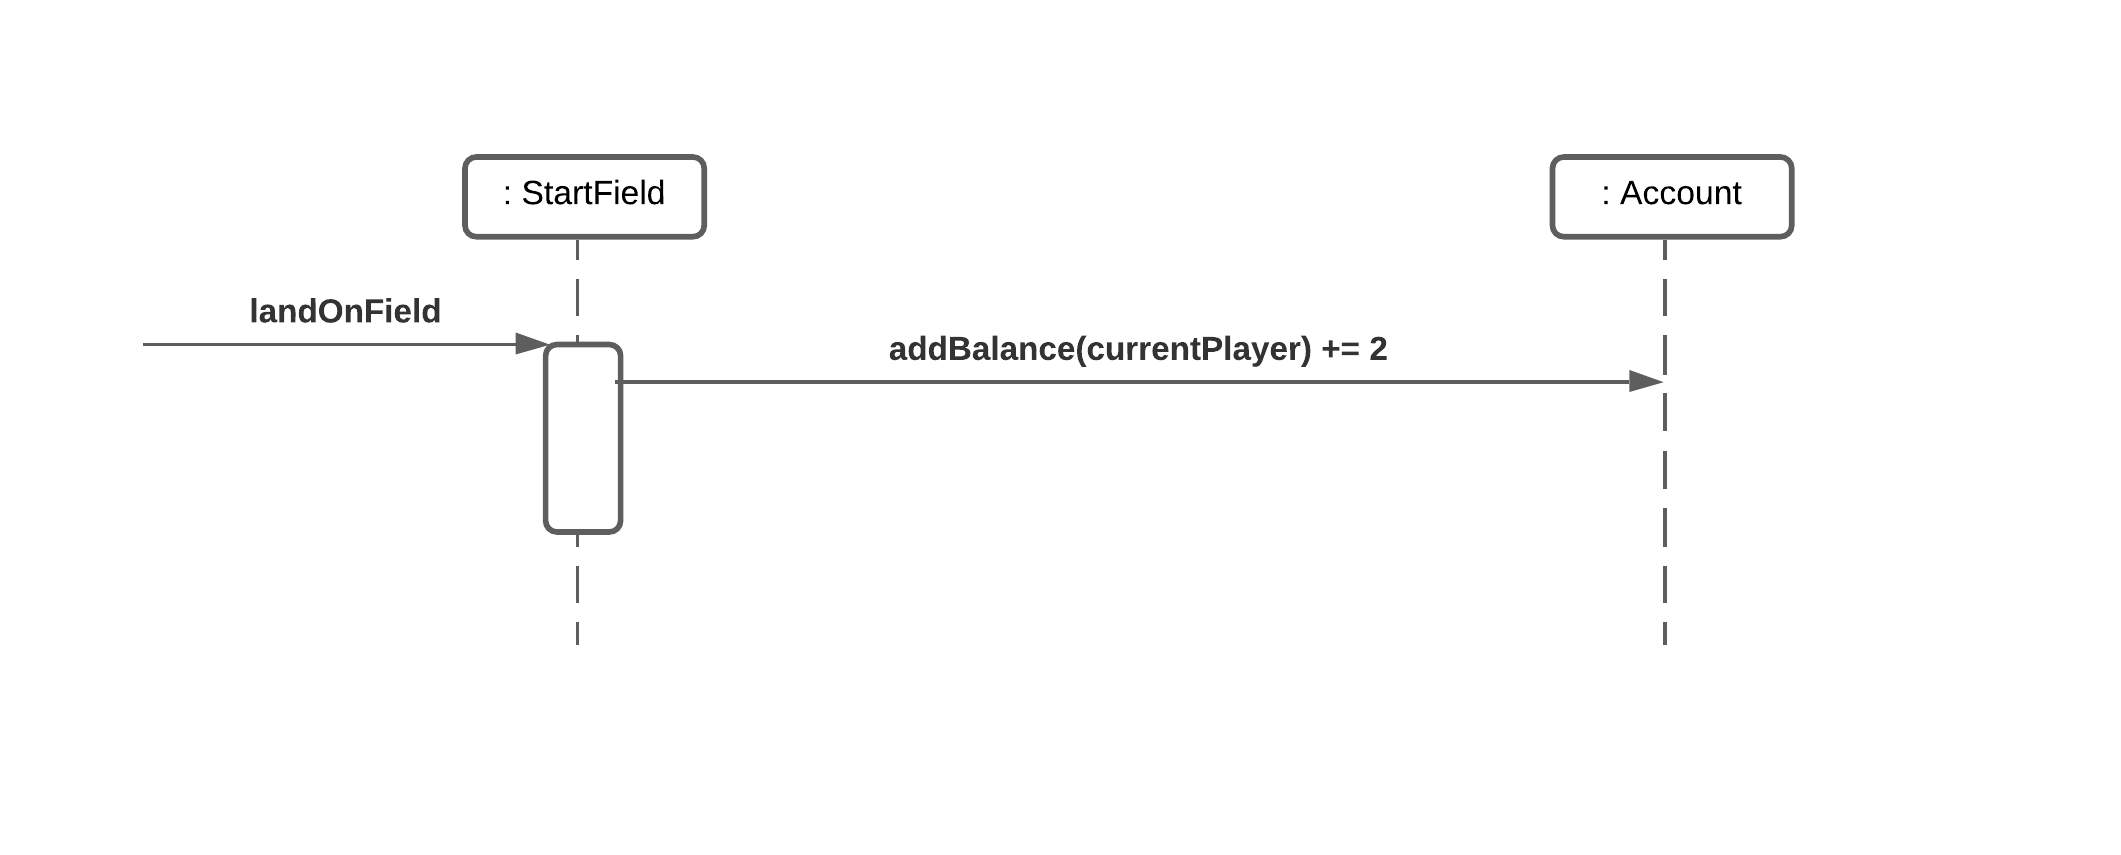
\includegraphics[width=0.9\textwidth]{Report/figures/Sekvensdiagram_StartField.png}~\\[0cm]
Figur 5.1.6. StartField over polymorphism af metoden landOnField for ChanceField.
\subsection{Designmønster GRASP}
I dette afsnit beskriver vi kort, hvordan vores design har overholdt GRASP principper. Her refereres der til designklassediagrammet (se figur 5.2.1) uden at danne en fyldestgørende beskrivelse af dette diagram. For en fyldestgørende beskrivelse, se afsnit 5.3.
\subsection{Designklassediagram}
\begin{center}
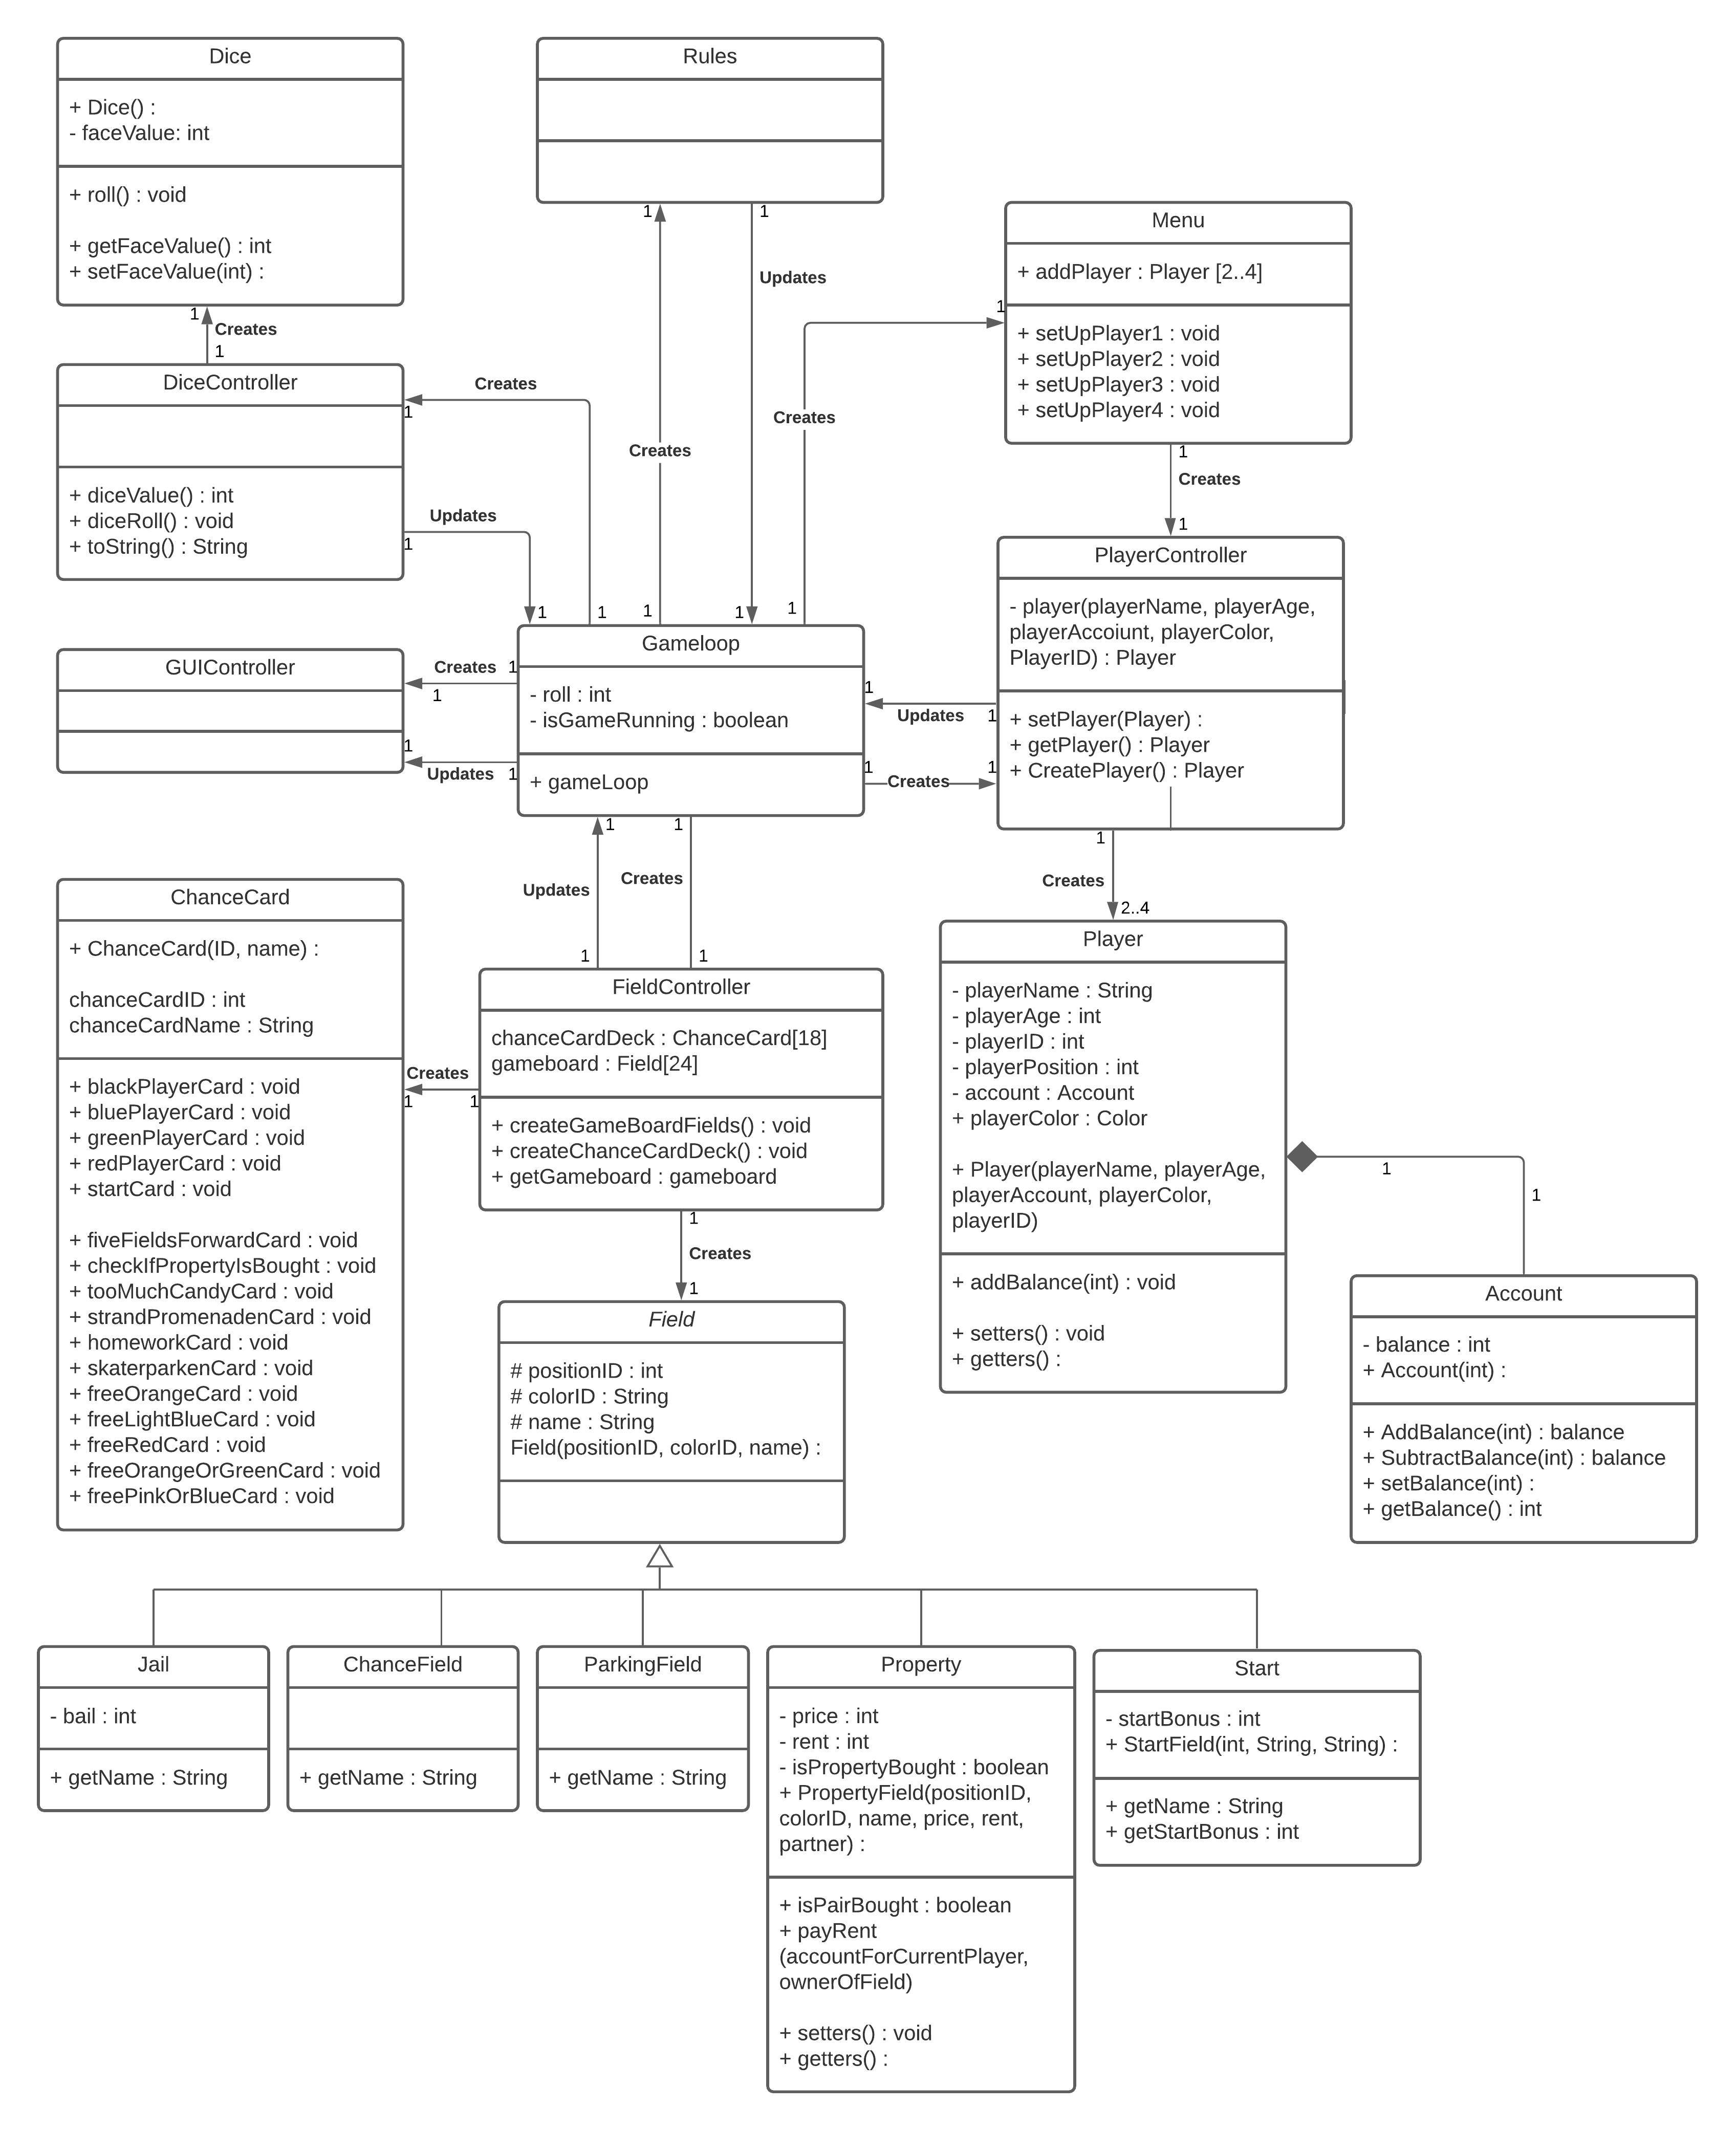
\includegraphics[width=1\textwidth]{Report/figures/Class Diagram.png}~\\[0cm]
\end{center}
Figur 5.2.1. Designklassediagram over Monopoly Junior spillet.
\end{flushleft}
\thispagestyle{fancy}

\newpage
\section{Implementering}
\begin{flushleft} % sætter tekststarten i venstre marginside.

\subsection{Kode udskrift 1}

I Latex skiftes automatisk linje når man skriver en lang sætning på den her måde, som I kan se.

\addlinespace % linjeskifts mellemrum

Indsæt grafer:
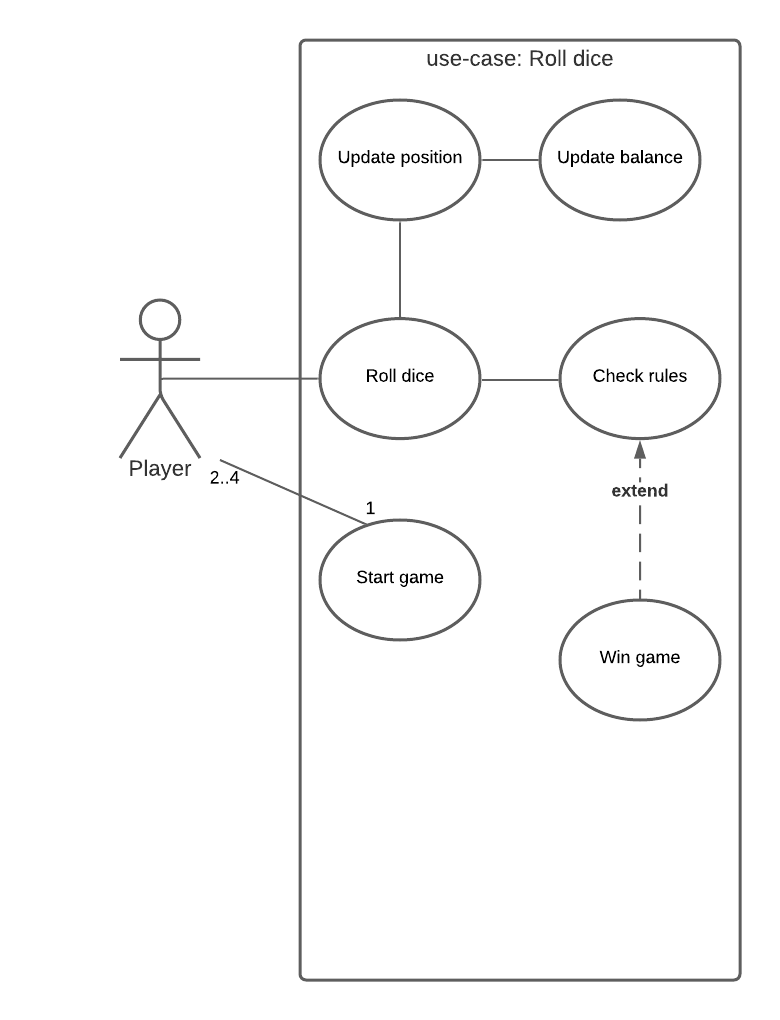
\includegraphics[width=1\textwidth]{Report/figures/Use case diagram CDIO del3.png}~\\[1cm]


\end{flushleft}
\thispagestyle{fancy}

\newpage
\section{Test}
\begin{flushleft} % sætter tekststarten i venstre marginside.

\subsection{kodeudskrift 2}

I Latex skiftes automatisk linje når man skriver en lang sætning på den her måde, som I kan se.

\addlinespace % linjeskifts mellemrum

Indsæt grafer:
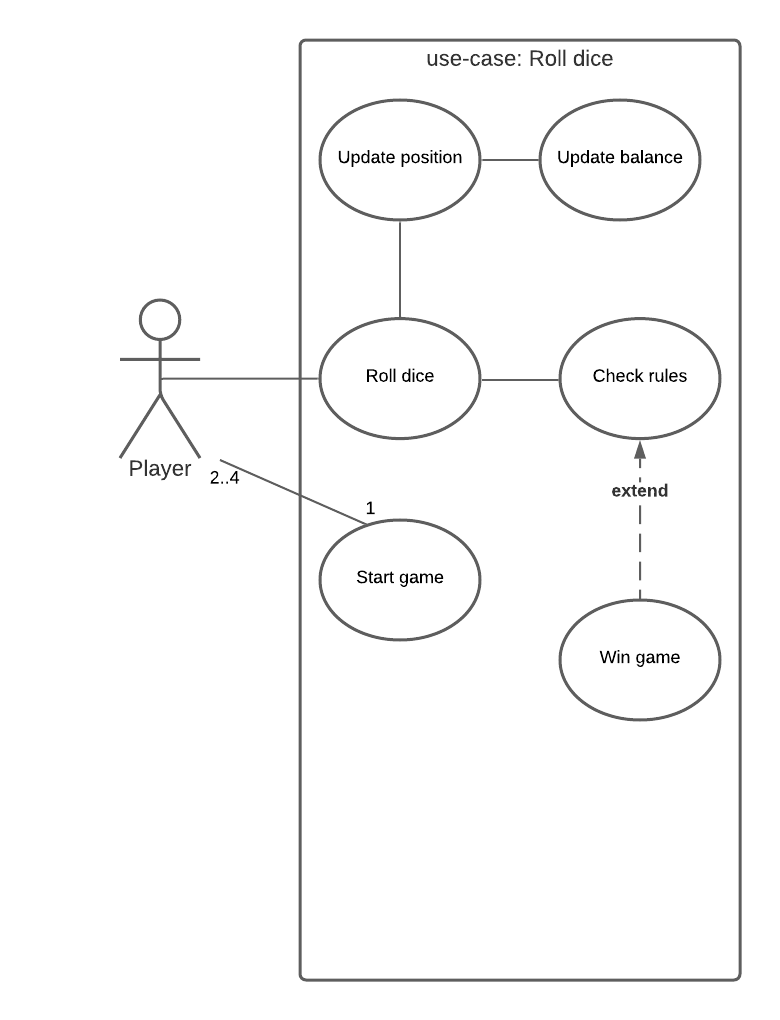
\includegraphics[width=1\textwidth]{Report/figures/Use case diagram CDIO del3.png}~\\[1cm]


\end{flushleft}
\thispagestyle{fancy}

\newpage
\section{Projektplanlægning}
\input{Report/sources/7_Projektplanlægning}
\thispagestyle{fancy}

\newpage
\section{Brugerguide}
\begin{document}
\begin{flushleft}
 \doublespacing   
    \subsection{How to import project from GitHub}
    1. Open project from GitHub\\
    2. Open "Code" dropdown menu and click "Download ZIP"\\
    \vspace{5mm}
    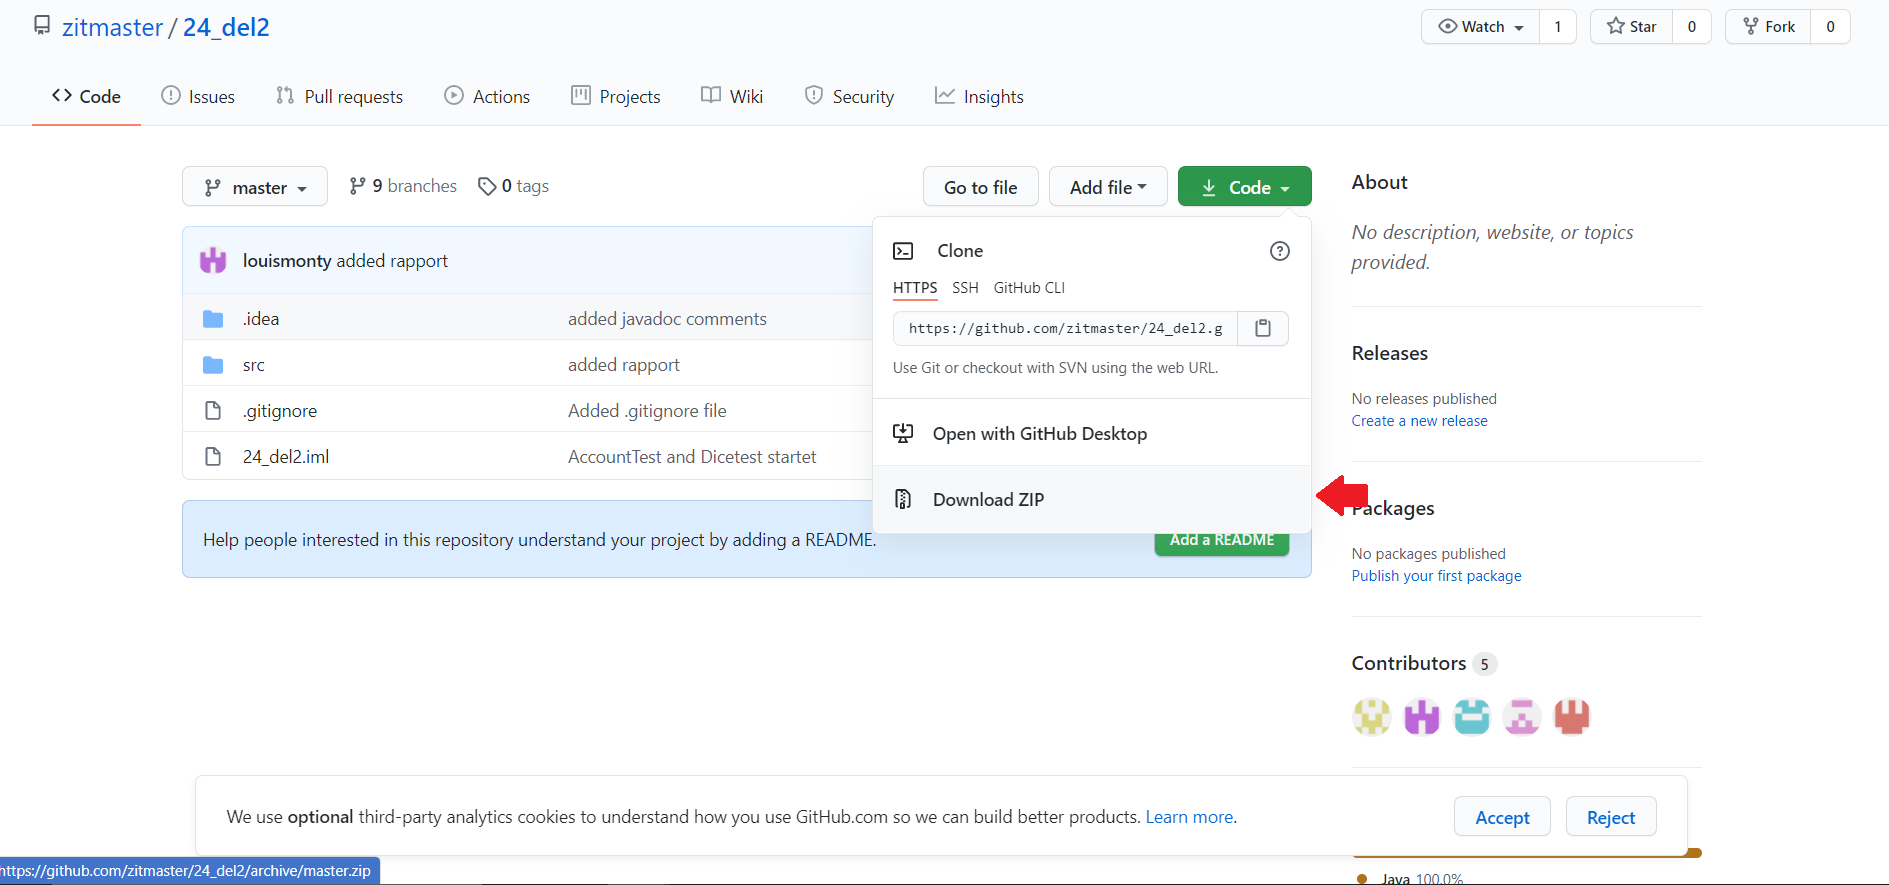
\includegraphics[width=16.5cm]{Report/root/step1.png}\\
    3. Unzip/extract downloaded .zip file to an arbitrary folder\\
    \newpage
    4. Copy the path from unzipped/extracted folder\\
    \begin{verbatim}
    Example: C:\Users\Simon\Dokumenter\Forprojects\24_del2-master\    
    \end{verbatim}
    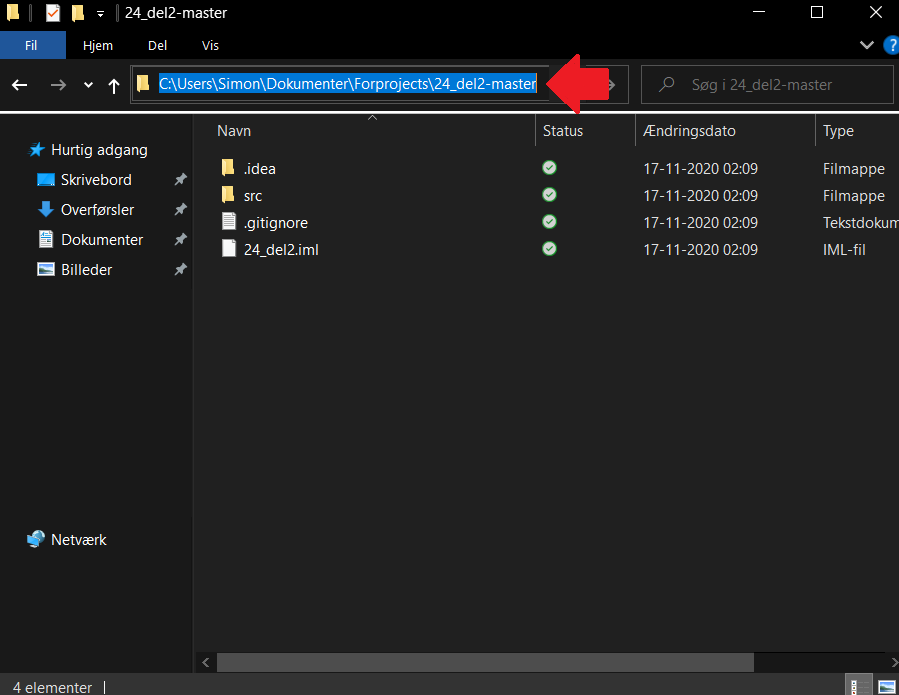
\includegraphics[width=16.5cm]{Report/root/step2.png}\\
    5. Open IntelliJ\\
    \newpage
    6. Click open or Import (if welcome page not shown, skip this step)\\
    \vspace{5mm}
    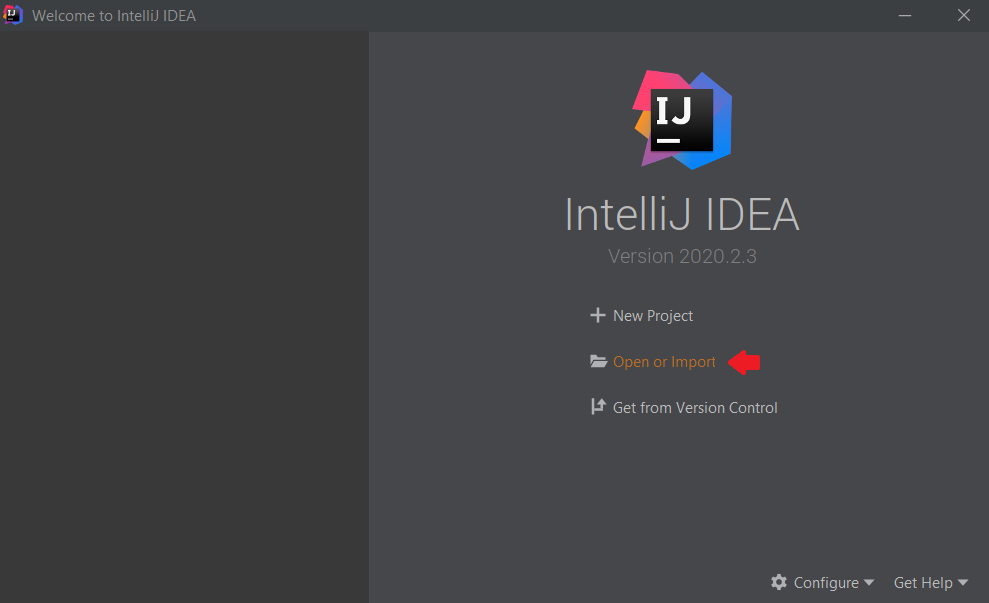
\includegraphics[width=16.5cm]{Report/root/step3.1.png}\\
    7. Click "File" then "Open" (If welcome page was shown, skip this step)\\
    \vspace{5mm}
    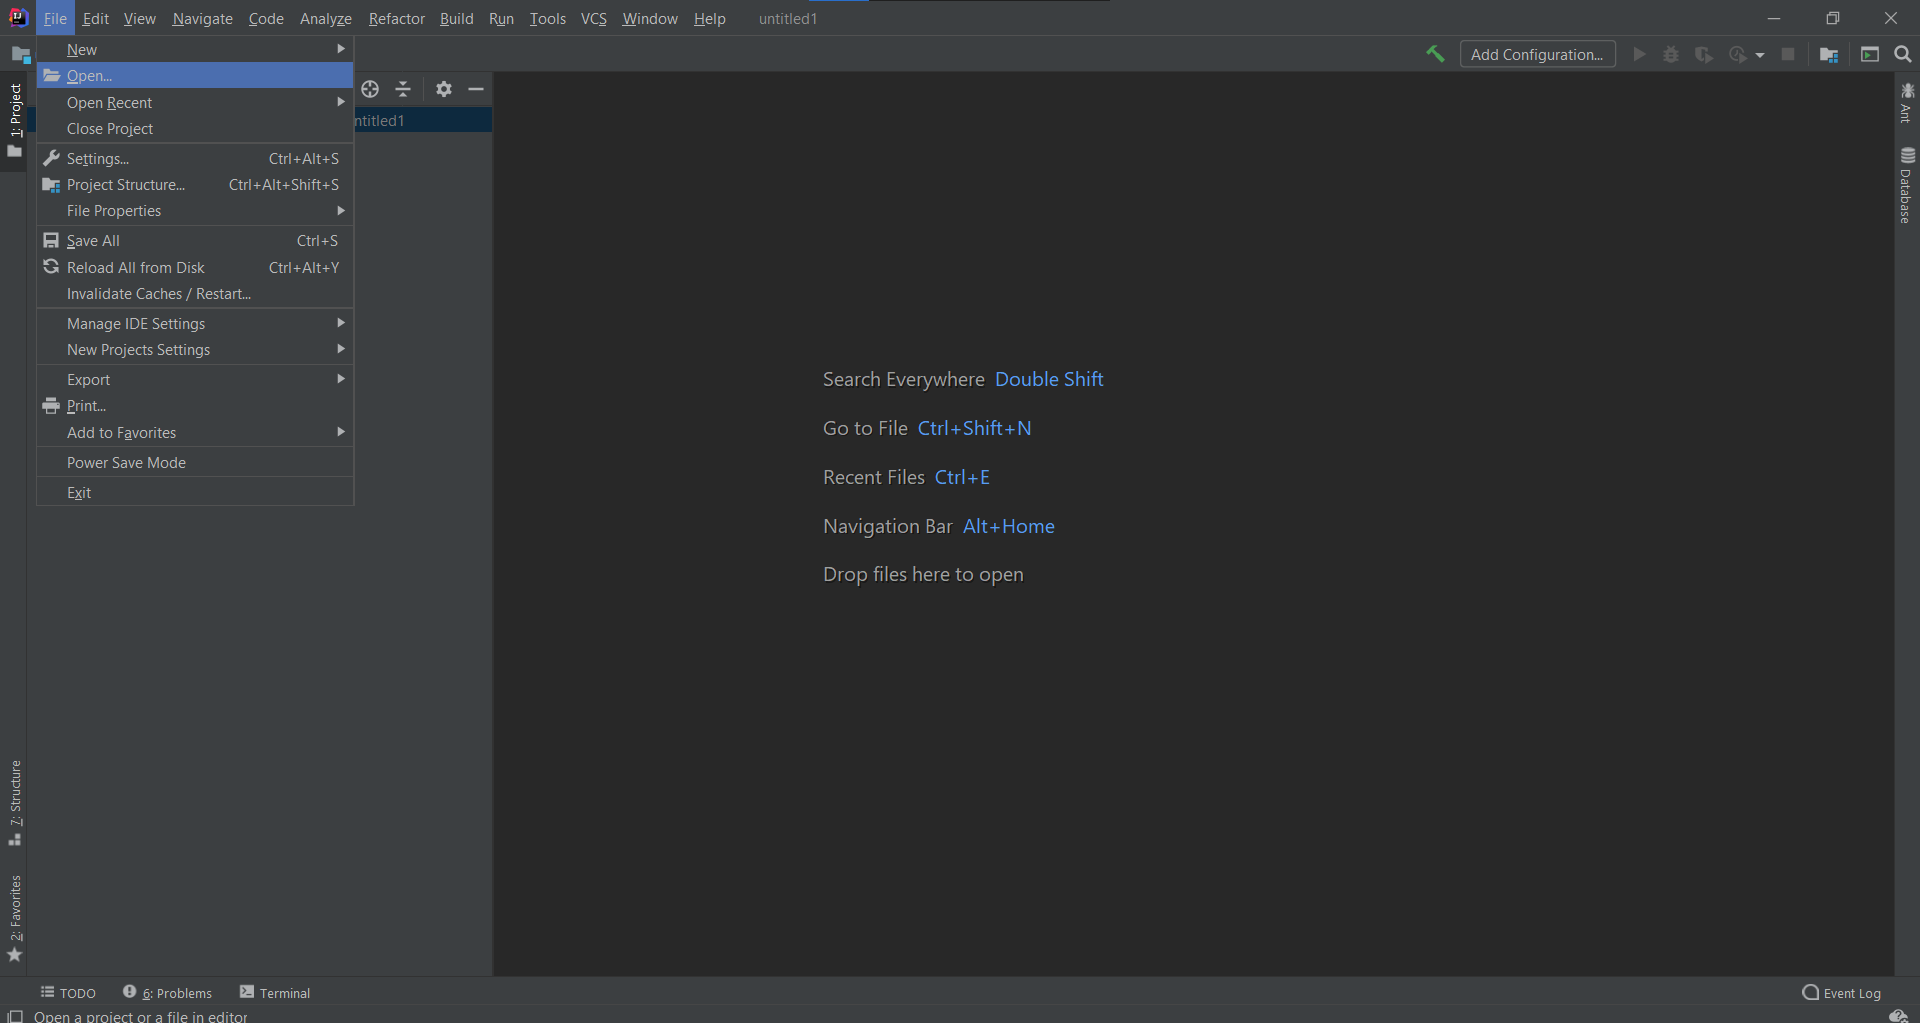
\includegraphics[width=16.5cm]{Report/root/step3.2.png}\\
    \newpage
    8. Paste the copied path and hit enter\\
    \vspace{5mm}
    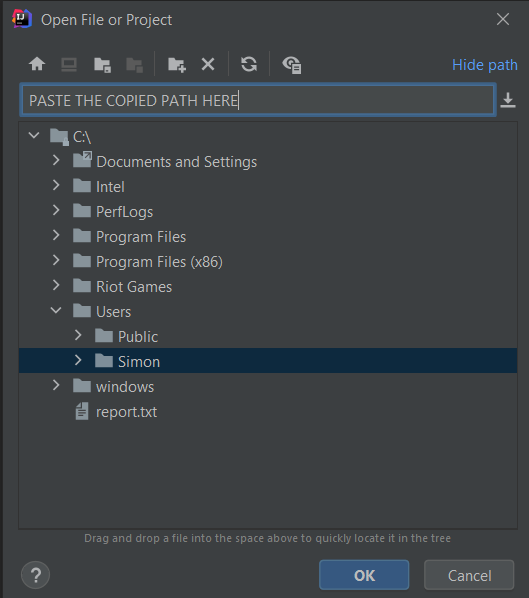
\includegraphics[width=16.5cm]{Report/root/step4.png}\\
    Now the project should be shown and ready to run\\
    \newpage
    It should look like this\\
    \vspace{5mm}
    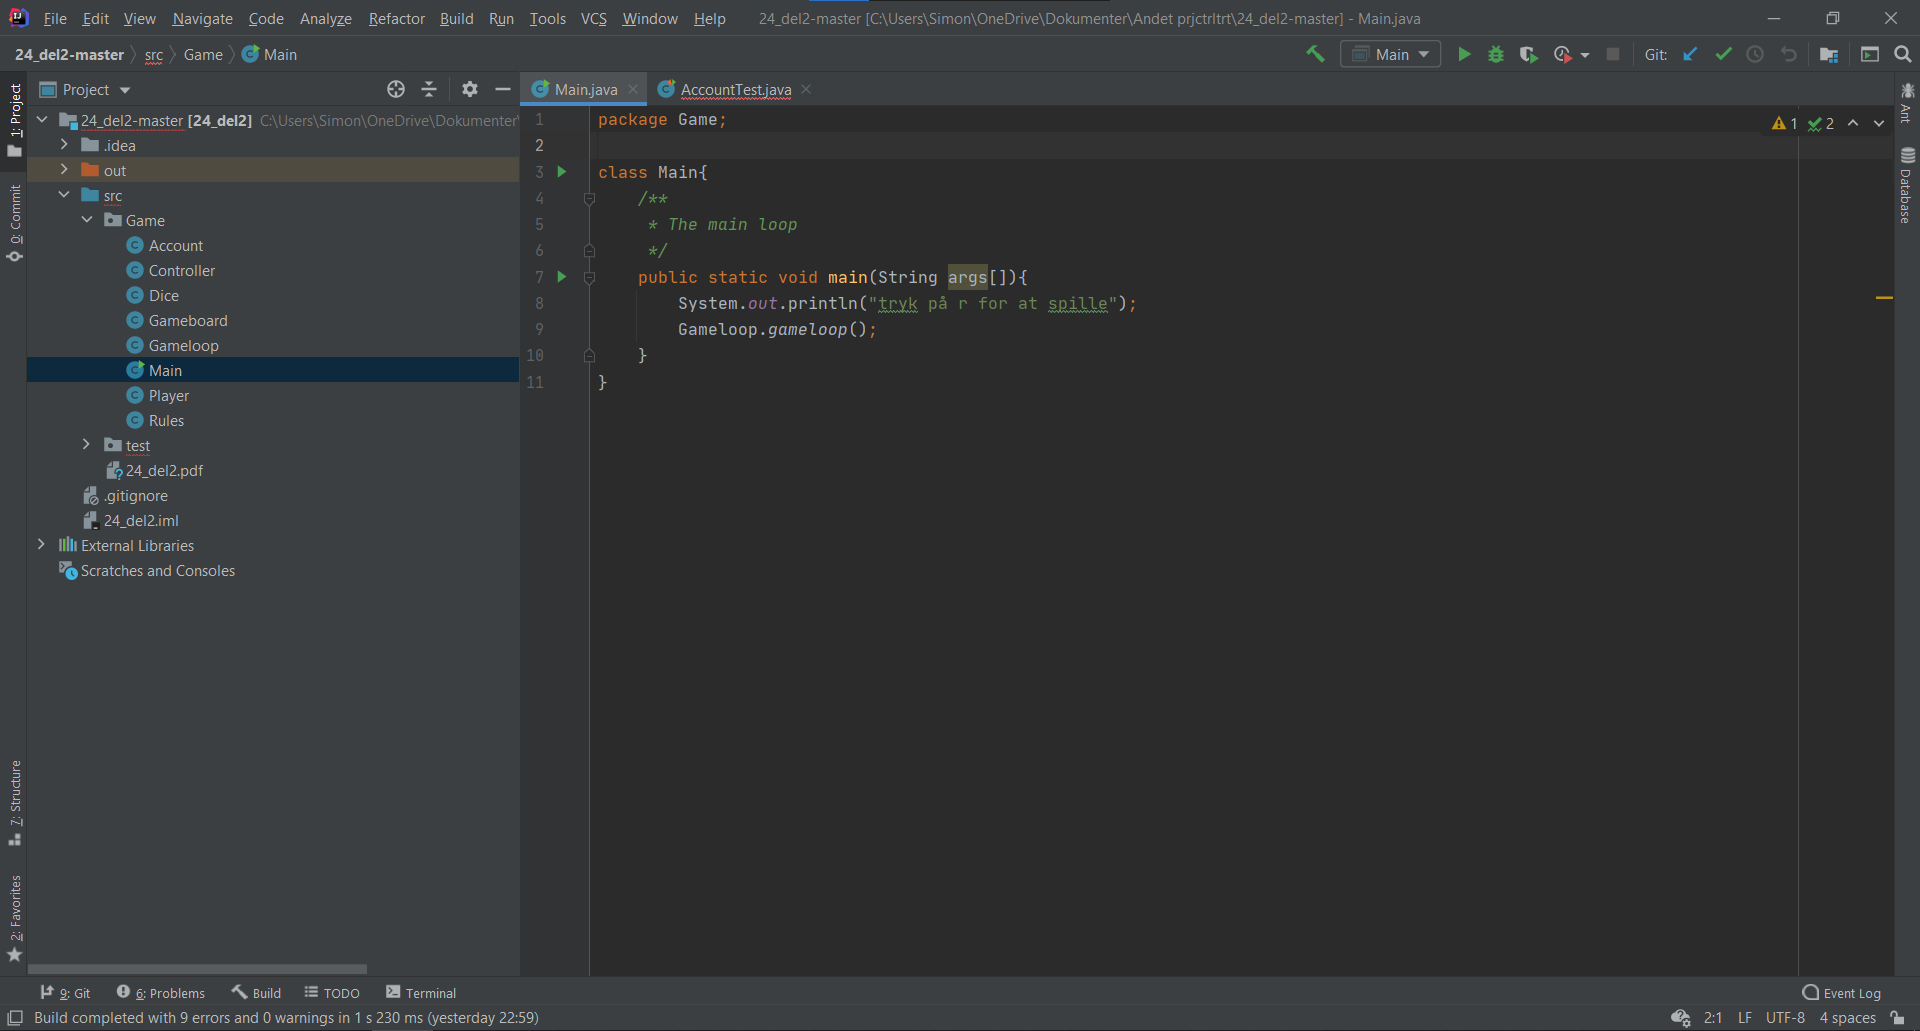
\includegraphics[width=16.5cm]{Report/root/step5.png}\\
    9. To run/execute the project press "Shift" + "F10"

    
    
\end{flushleft}
\end{document}
\thispagestyle{fancy}

\newpage
\section{Konklusion}
\begin{flushleft} % sætter tekststarten i venstre marginside.

\subsection{kodeudskrift 2}

I Latex skiftes automatisk linje når man skriver en lang sætning på den her måde, som I kan se.

\addlinespace % linjeskifts mellemrum

Indsæt grafer:
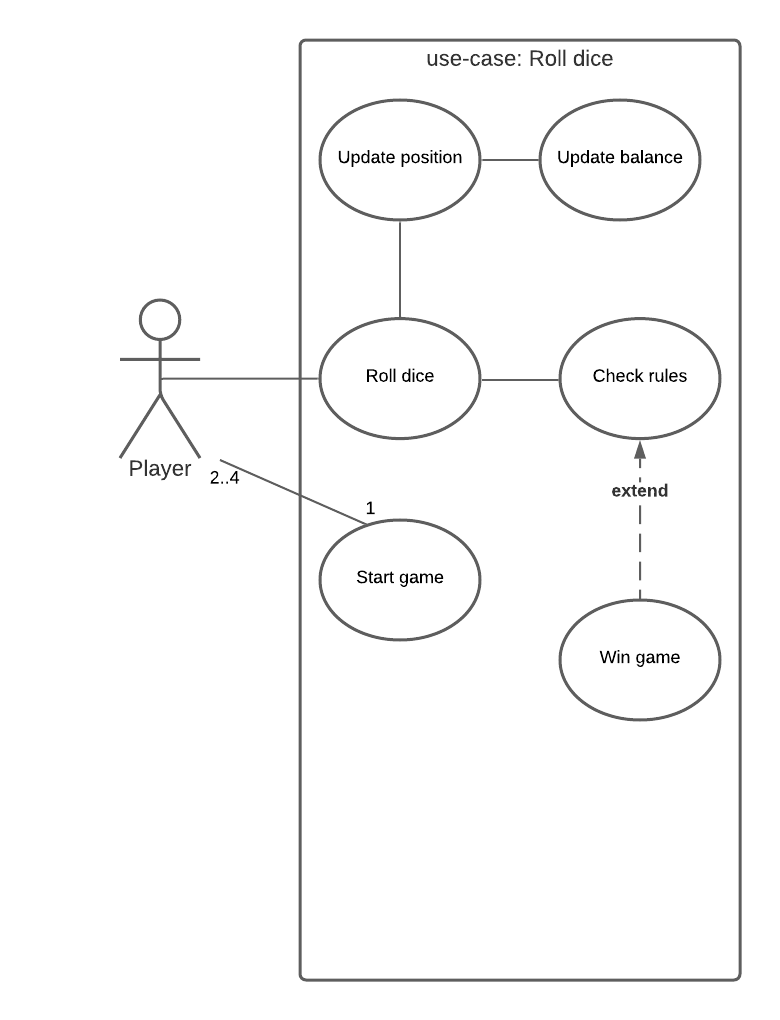
\includegraphics[width=1\textwidth]{Report/figures/Use case diagram CDIO del3.png}~\\[1cm]


\end{flushleft}
\thispagestyle{fancy}

\newpage
\begin{flushleft}
\section{Tegn og ordforklaring}
\end{flushleft}
\begin{flushleft}
\begin{tabular}{ | c | c | } 
\hline
Tegn / ord & Forklaring \\ 
\hline
UTF-8 & Indkodning af unicode tegnsættet for at kunne visualisere symboler. \\ 
\hline
IntelliJ & IDE, der understøttet flere forskellige programmeringssprog, inkl. Java. \\ 
\hline
Git & Versionsstyringsværktøj. \\ 
\hline
Overleaf & Online tekstredigeringsværktøj, der følger LaTeX framework. \\ 
\hline
Maven & Værktøj til at organisere java-projekter og tests. \\ 
\hline
JUnit & Framework til at teste forskellige units i Java. \\ 
\hline
GUI & Graphical User Interface: Den visuelle del af programmet. \\ 
\hline
 
\hline
\end{tabular}

\end{flushleft}
\thispagestyle{fancy}

\newpage
\section{Litteraturliste}
\begin{flushleft}

\end{flushleft}

\newpage
\section{Bilag}
\label{endOfText}
\label{endOfDoc}



\end{document}